As stated previously, it is necessary to integrate the developed ontology with a Java application.
The developed Java application will be used to manage athletes' training sessions data and provide feedback on their posture.
The ontology will be used to infer the correct execution of an weightlifting exercise based on the data received from training.

Displayed in Figure~\ref{fig:ont_int} is part of the application behavior.
Starting with a click event, an XML parsing process is initiated to convert rules into an SQWRL query format.
After that, is established a connection to an SQL database to retrieve the athlete's training data.
Then is performed a conversion of the ontology OWLModel to an OntModel for it to be used with the SQWRL query engine.
In the created OntModel is created an individual to hold the athlete's training session data that will be used for the inference process.
Because this is done in a "temporary" model, none of these actions will have any effect on the developed ontology.
Finally, the inference process takes place with the execution of each query through the Query Engine.
In the end of this process the results are displayed, telling the athlete which parts of the exercise were well done and not well done.

\begin{figure}[h]
	\centering
		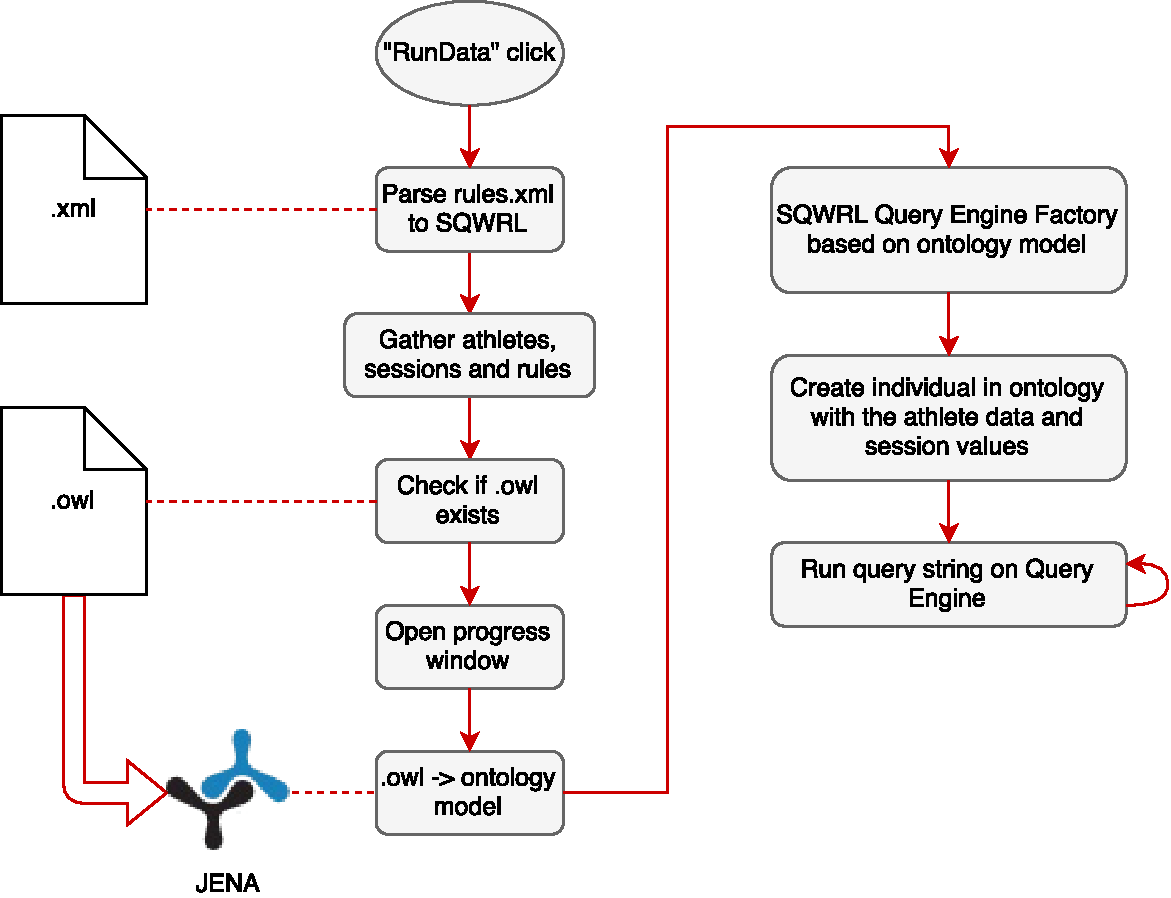
\includegraphics[width=1.00\textwidth]{Images/integration.pdf}
	\caption{Ontology integration.}
	\label{fig:ont_int}
\end{figure}

The selected API provides some methods that make the integration more easy.
The \textit{createJenaOWLModelFromURI()} method performs the construction of an OntModel from an OWLModel.
There is also the \textit{create()} method that is called on a \textbf{P3SQWRLQueryEngineFactory} object to create the query engine and this has the \textit{runSQWRLQuery()} method that is used to execute the queries and return the result. 
